\section{Contratación pública (SECOP)}

Este es el primero de tres capítulos dedicados, cada uno, a una de las dimensiones de la participación del egresado. Lo abrimos con la contratación pública porque es la de cobertura más completa ---el enlace con el SECOP Integrado se hace de forma exacta por documento--- y la más frecuente: \textbf{42.889 graduados}, alrededor del 24,6\,\% de los 174.685 egresados de las seis sedes, figuran como contratistas del Estado, con \textbf{347.097 contratos} a su nombre. La pregunta de este capítulo no es ya \emph{cuántos} contratan, sino \emph{qué}, \emph{cómo}, \emph{con quién}, \emph{desde qué carrera} y \emph{en qué territorio} lo hacen. Para responderla cruzamos las dimensiones que el SECOP Integrado expone por contrato ---tipo de contrato, modalidad de contratación y nivel de la entidad--- con la carrera y la sede de origen del graduado.

\subsection{Tipo de contrato}
La Tabla~\ref{tab:secop_tipo} no deja lugar a dudas: la contratación del egresado es, de manera abrumadora, prestación de servicios. Este único tipo concentra el \textbf{92,7\,\%} de los 347.097 contratos (321.643), dejando a los demás ---obra, suministro, consultoría, interventoría--- en posiciones marginales, cada uno por debajo del 2\,\%. El dato retrata con fidelidad la forma dominante en que el profesional colombiano se vincula con el Estado: el clásico contrato de prestación de servicios de persona natural, mediante el cual el egresado aporta su trabajo profesional sin constituir empresa. La Figura~\ref{fig:secoptipo} muestra, en cambio, que cuando se mira el \emph{valor} y no el conteo, la obra y otros tipos de contrato ganan peso, pues se trata de contratos individualmente mucho más cuantiosos aunque mucho menos numerosos.

\begin{table}[H]\centering\footnotesize
\caption{Contratación de los graduados por \textbf{tipo de contrato} (SECOP Integrado).}\label{tab:secop_tipo}
\begin{tabular}{lrrrr}
\toprule
\rowcolor{ustaazul}\textbf{\color{white}Tipo de contrato} & \textbf{\color{white}Proveedores} & \textbf{\color{white}Contratos} & \textbf{\color{white}\% contr.} & \textbf{\color{white}Valor} \\
\midrule
Prestación De Servicios & 41,260 & 321,643 & 92.7 & \$22.8 bill. \\
Obra & 1,257 & 6,647 & 1.9 & \$3.9 bill. \\
Suministro & 1,046 & 4,610 & 1.3 & \$308.2 mil mill. \\
Consultoría & 915 & 2,377 & 0.7 & \$103.8 mil mill. \\
Otro Tipo De Contrato & 811 & 2,337 & 0.7 & \$4.6 bill. \\
Compraventa & 500 & 2,319 & 0.7 & \$347.4 mil mill. \\
Decreto 092 De 2017 & 725 & 2,164 & 0.6 & \$72.9 mil mill. \\
Interventoría & 550 & 1,920 & 0.6 & \$141.6 mil mill. \\
Arrendamiento & 427 & 916 & 0.3 & \$27.2 mil mill. \\
Arrendamiento De Inmuebles & 174 & 728 & 0.2 & \$41.3 mil mill. \\
\bottomrule
\end{tabular}
\\[2pt]{\scriptsize\color{ustagris} Ordenado por número de contratos. El valor está sesgado por pocos megacontratos de fiducia.}
\end{table}

\begin{figure}[H]\centering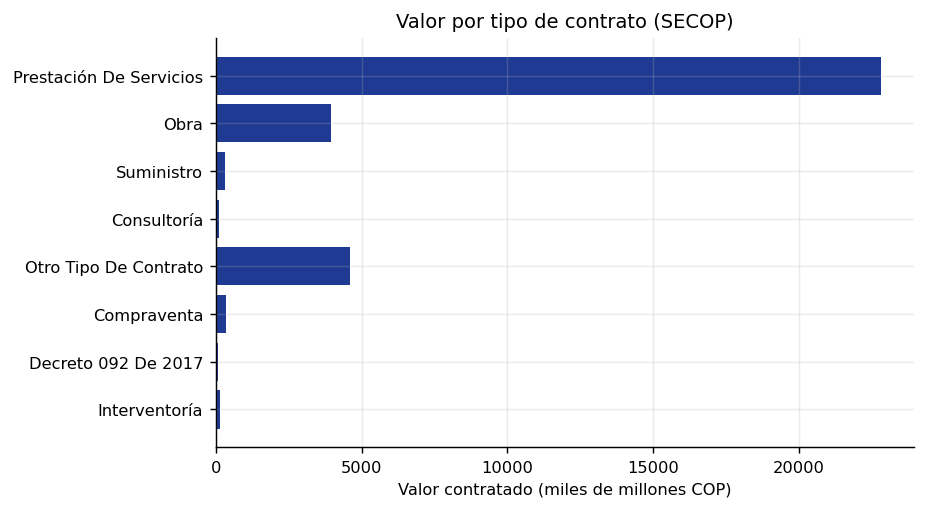
\includegraphics[width=0.74\linewidth]{figs_cruce/S1_secop_tipo.png}
\caption{Valor contratado por tipo de contrato. La obra y otros tipos de contrato, pese a ser minoritarios en número, concentran montos elevados.}\label{fig:secoptipo}\end{figure}

\subsection{Modalidad de contratación}
La modalidad de contratación (Tabla~\ref{tab:secop_modalidad}) confirma la lectura anterior desde el ángulo del procedimiento. La \textbf{contratación directa} y el \textbf{régimen especial} ---las vías habituales de los contratos de prestación de servicios--- son las que vinculan al grueso de los egresados, mientras que la \textbf{licitación pública}, reservada a los contratos de mayor cuantía, concentra una porción desproporcionada del valor (el 54,6\,\%) pese a su menor frecuencia. El egresado-contratista típico no compite en grandes licitaciones: es contratado de forma directa o por régimen especial para prestar un servicio profesional, y solo un puñado de vínculos pasa por la licitación que mueve las sumas mayores.

\begin{table}[H]\centering\footnotesize
\caption{Contratación de los graduados por \textbf{modalidad de contratación}.}\label{tab:secop_modalidad}
\begin{tabular}{lrrrr}
\toprule
\rowcolor{ustaazul}\textbf{\color{white}Modalidad} & \textbf{\color{white}Proveedores} & \textbf{\color{white}Contratos} & \textbf{\color{white}Valor} & \textbf{\color{white}\% valor} \\
\midrule
Licitación Pública & 239 & 790 & \$36.0 bill. & 54.6 \\
Contratación Régimen Especial & 3,431 & 14,279 & \$11.0 bill. & 16.7 \\
Contratación Directa & 26,211 & 166,002 & \$6.4 bill. & 9.7 \\
Régimen Especial & 7,279 & 29,195 & \$6.1 bill. & 9.3 \\
Contratación Directa (Ley 1150 De 2007) & 26,826 & 117,781 & \$4.4 bill. & 6.7 \\
Selección Abreviada De Menor Cuantía (Ley 1150 De 2007) & 528 & 2,373 & \$423.3 mil mill. & 0.6 \\
Contratación Régimen Especial (Con Ofertas) & 51 & 112 & \$247.0 mil mill. & 0.4 \\
Selección Abreviada De Menor Cuantía & 111 & 588 & \$228.9 mil mill. & 0.3 \\
\bottomrule
\end{tabular}
\end{table}

\subsection{Nivel de la entidad contratante}
Aquí emerge uno de los contrastes más instructivos del capítulo. Como muestran la Tabla~\ref{tab:secop_nivel} y la Figura~\ref{fig:secopnivel}, el \textbf{67,8\,\%} de los contratos de los graduados se firma con entidades del \textbf{orden territorial} (gobernaciones, alcaldías, entidades departamentales y municipales), pero esos contratos representan apenas el \textbf{38,1\,\%} del valor. A la inversa, las entidades del \textbf{orden nacional} suscriben solo el 32,2\,\% de los contratos pero acumulan el \textbf{61,9\,\%} del valor. Dicho de otro modo: el egresado trabaja, en su día a día, sobre todo para el Estado local ---que es quien le da dos de cada tres contratos---, mientras que las sumas verdaderamente grandes provienen de los vínculos con el nivel nacional.

\begin{table}[H]\centering\footnotesize
\caption{Contratación de los graduados por \textbf{nivel de la entidad} contratante.}\label{tab:secop_nivel}
\begin{tabular}{lrrrr}
\toprule
\rowcolor{ustaazul}\textbf{\color{white}Nivel de la entidad} & \textbf{\color{white}Contratos} & \textbf{\color{white}\% contratos} & \textbf{\color{white}Valor} & \textbf{\color{white}\% valor} \\
\midrule
Nacional & 111,804 & 32.2 & \$40.8 bill. & 61.9 \\
Territorial & 235,175 & 67.8 & \$25.1 bill. & 38.1 \\
(sin dato) & 118 & 0.0 & \$1.9 mil mill. & 0.0 \\
\bottomrule
\end{tabular}
\end{table}

\begin{figure}[H]\centering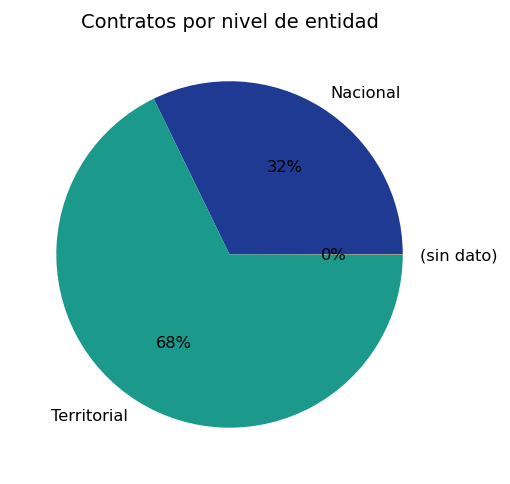
\includegraphics[width=0.50\linewidth]{figs_cruce/S3_secop_nivel.png}
\caption{Distribución de los contratos de los graduados según el nivel de la entidad contratante.}\label{fig:secopnivel}\end{figure}

\subsection{Concentración del valor en pocos contratos}
Antes de leer cualquier cifra de valor agregado conviene una cautela estadística. El valor total contratado ---del orden de \$65,9 billones--- está \textbf{fuertemente dominado por unos pocos atípicos}: el 10\,\% de proveedores de mayor monto concentra el \textbf{76,6\,\%} de todo el valor, y un \emph{único} documento aporta por sí solo \$22,2 billones, más de un tercio del total. Excluyéndolo, el agregado cae a \$43,7 billones. La mediana, en cambio, se sitúa en unos \textbf{\$113 millones} por proveedor, una cifra mucho más representativa del contratista real y dos órdenes de magnitud por debajo de los grandes montos que inflan la suma.

\begin{cajaobs}
Las sumas de valor deben leerse con prudencia. Un solo documento aporta más de un tercio del valor agregado, casi con certeza una colisión de identidad entre una cédula de graduado y una estructura de gran tamaño, o un contrato administrado a nombre de persona natural. Por ello, a lo largo del capítulo se privilegian las medidas robustas ---el número de proveedores, el número de contratos y la mediana de valor--- sobre las sumas, sensibles a estos atípicos. Un grupo reducido de megacontratos basta para desplazar el agregado en varios billones de pesos, de modo que cualquier comparación entre carreras o territorios que descanse en valores totales arrastra ese sesgo; la mediana, insensible a los extremos, ofrece el retrato fiel del egresado-contratista. La verificación de los megacontratos por documento queda como tarea de depuración pendiente.
\end{cajaobs}

\subsection{Contratación por carrera}
La Tabla~\ref{tab:secop_carrera} ordena los programas por número de graduados proveedores y revela una jerarquía nítida. El \textbf{Derecho} domina con holgura la contratación pública: \textbf{8.284} de sus egresados son proveedores del Estado y acumulan \textbf{74.243} contratos, una preeminencia coherente con la naturaleza jurídica de buena parte de la actividad estatal. Le siguen la Especialización en Derecho Administrativo (3.317 proveedores), la \textbf{Ingeniería Civil} (2.159) y la \textbf{Arquitectura} (1.882), volcadas a la obra y la consultoría públicas, y más atrás la \textbf{Odontología} (907), cuya presencia delata la contratación de servicios de salud por parte de entidades territoriales. Es revelador, además, que sean las \textbf{especializaciones} ---en particular la Especialización en Derecho Administrativo, con una mediana de \$173,9 millones--- las que exhiben las medianas de valor más altas: el posgrado no solo da acceso a la contratación, sino a contratos de mayor cuantía individual.

\begin{table}[H]\centering\footnotesize
\caption{Contratación pública por \textbf{carrera}: programas con más graduados proveedores.}\label{tab:secop_carrera}
\begin{tabular}{lrrrr}
\toprule
\rowcolor{ustaazul}\textbf{\color{white}Programa (carrera)} & \textbf{\color{white}Proveedores} & \textbf{\color{white}Contratos} & \textbf{\color{white}Valor (mediana)} & \textbf{\color{white}Valor total} \\
\midrule
Derecho & 8,284 & 74,243 & \$147.7 mill. & \$14.1 bill. \\
Especializacion En Derecho Admin & 3,317 & 33,795 & \$173.9 mill. & \$1.1 bill. \\
Ingenieria Civil & 2,159 & 14,884 & \$114.6 mill. & \$2.5 bill. \\
Arquitectura & 1,882 & 13,333 & \$77.5 mill. & \$4.8 bill. \\
Economia & 1,230 & 9,468 & \$136.3 mill. & \$22.7 bill. \\
Contaduria Publica & 1,227 & 8,868 & \$77.0 mill. & \$339.3 mil mill. \\
Psicologia & 1,221 & 8,811 & \$102.2 mill. & \$8.4 bill. \\
Especializacion En Auditoria De  & 1,090 & 10,734 & \$109.6 mill. & \$360.9 mil mill. \\
Negocios Internacionales & 1,068 & 6,303 & \$67.1 mill. & \$180.8 mil mill. \\
Cultura Fisica, Deporte Y Recrea & 1,008 & 6,852 & \$74.9 mill. & \$158.9 mil mill. \\
Odontologia & 907 & 5,410 & \$48.9 mill. & \$2.8 bill. \\
Ingenieria Ambiental & 761 & 5,203 & \$120.2 mill. & \$148.8 mil mill. \\
\bottomrule
\end{tabular}
\\[2pt]{\scriptsize\color{ustagris} Programa principal de cada proveedor. Ordenado por nº de proveedores. La mediana evita el sesgo de los megacontratos.}
\end{table}

\subsection{Objeto del contrato (UNSPSC)}
El tipo y la modalidad describen la \emph{forma} del contrato, pero no su \emph{objeto}. Para saber qué se contrata realmente hay que recurrir al clasificador internacional de bienes y servicios UNSPSC, que el SECOP Integrado no expone pero el SECOP~II sí. Cruzando a los graduados con el SECOP~II ---que cubre los contratos electrónicos, alrededor del 39\,\% del total--- se recupera el código UNSPSC de \textbf{136.800} de sus contratos. La Tabla~\ref{tab:secop_unspsc} muestra el resultado, y de entrada confirma una sospecha: la administración pública \emph{uniformiza}. El \textbf{79,3\,\%} de los contratos cae en una única categoría genérica de apoyo profesional y gestión ---encabezada por el código 80111600, ``servicios de personal''---, con la que el Estado rotula casi cualquier contrato de prestación de servicios, sea quien sea el contratista. El UNSPSC, al igual que el tipo de contrato, está dominado por ese cajón de sastre administrativo.

\begin{table}[H]\centering\footnotesize
\caption{Objeto contratado por los graduados según el clasificador \textbf{UNSPSC} (SECOP II).}\label{tab:secop_unspsc}
\begin{tabular}{lrr}
\toprule
\rowcolor{ustaazul}\textbf{\color{white}Categoría de objeto (UNSPSC)} & \textbf{\color{white}Contratos (SECOP II)} & \textbf{\color{white}\%} \\
\midrule
Apoyo profesional y gestión & 108.535 & 79,3\% \\
Cívico y político & 6.518 & 4,8\% \\
Jurídico & 6.143 & 4,5\% \\
Salud & 4.075 & 3,0\% \\
Ingeniería y TI & 3.679 & 2,7\% \\
Otros & 2.266 & 1,7\% \\
Educación & 2.174 & 1,6\% \\
Ambiental & 1.358 & 1,0\% \\
Financiero y contable & 1.016 & 0,7\% \\
\bottomrule
\end{tabular}
\\[2pt]{\scriptsize\color{ustagris} Solo contratos electrónicos (SECOP II), ~38\% del total. El código 80111600 (apoyo profesional) domina la categoría genérica.}
\end{table}

La señal disciplinar, sin embargo, no desaparece: se esconde en el residuo especializado. Si se aparta esa categoría genérica y se observa solo el objeto \emph{específico} de los contratos, emerge con nitidez la firma de cada profesión, como revela la Figura~\ref{fig:secopunspsc}. La Odontología y la Especialización en Auditoría de Salud contratan salud ---el 85,5\,\% del objeto especializado de esta última---, la Contaduría Pública se concentra en lo financiero y contable (62,1\,\%), la Ingeniería Civil y la Arquitectura en lo técnico y de ingeniería (65,0\,\% y 59,9\,\% respectivamente), y el Derecho ---junto con la Especialización en Derecho Administrativo--- en lo jurídico (61,7\,\%) y los asuntos cívicos y políticos. El objeto del contrato traduce, así, con fidelidad la disciplina de origen del egresado: cuando el Estado contrata especializadamente, contrata exactamente aquello para lo que cada profesión forma.

\begin{figure}[H]\centering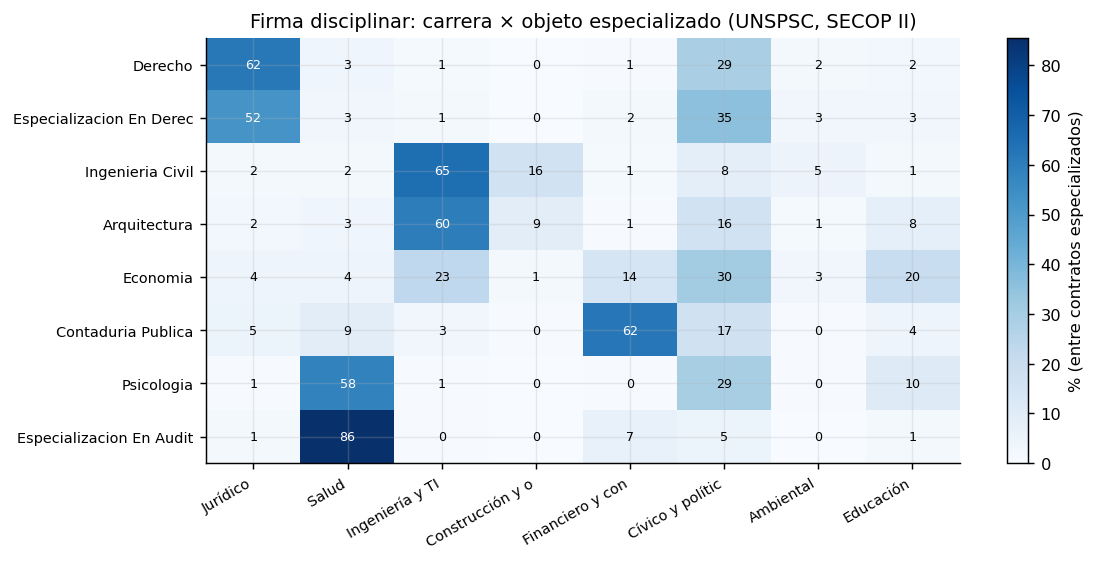
\includegraphics[width=0.94\linewidth]{figs_cruce/S6_secop_unspsc.png}
\caption{Objeto especializado de los contratos por carrera, según el código UNSPSC (\% sobre los contratos de cada carrera). Cada profesión deja su firma disciplinar una vez apartada la categoría genérica de apoyo profesional.}\label{fig:secopunspsc}\end{figure}

\subsection{Carrera y región de la contratación}
Superponer la carrera y el departamento de la entidad contratante (Figura~\ref{fig:secopcarrerareg}) combina las dos lecturas anteriores ---disciplinar y territorial--- en un solo mapa. El patrón general de arraigo regional se mantiene: cada profesión contrata sobre todo en los departamentos de sus sedes (Bogotá, Santander, Boyacá, Meta, Antioquia). Así, la Arquitectura concentra su contratación en Santander (36,8\,\%) y Boyacá (21,6\,\%), la Ingeniería Civil en Boyacá (31,3\,\%) y la Auditoría de Salud en Boyacá (33,5\,\%). Pero aparece un matiz disciplinar de interés: el \textbf{Derecho} muestra la mayor proyección nacional ---con el 42,6\,\% de sus contratos en Bogotá, sede de las entidades del orden nacional, y presencia repartida por Santander, Boyacá y el Meta---, mientras que profesiones más ligadas al territorio concentran su contratación en el departamento de su sede. La proyección nacional, así, no es homogénea: depende tanto de la disciplina como de la sede de origen.

\begin{figure}[H]\centering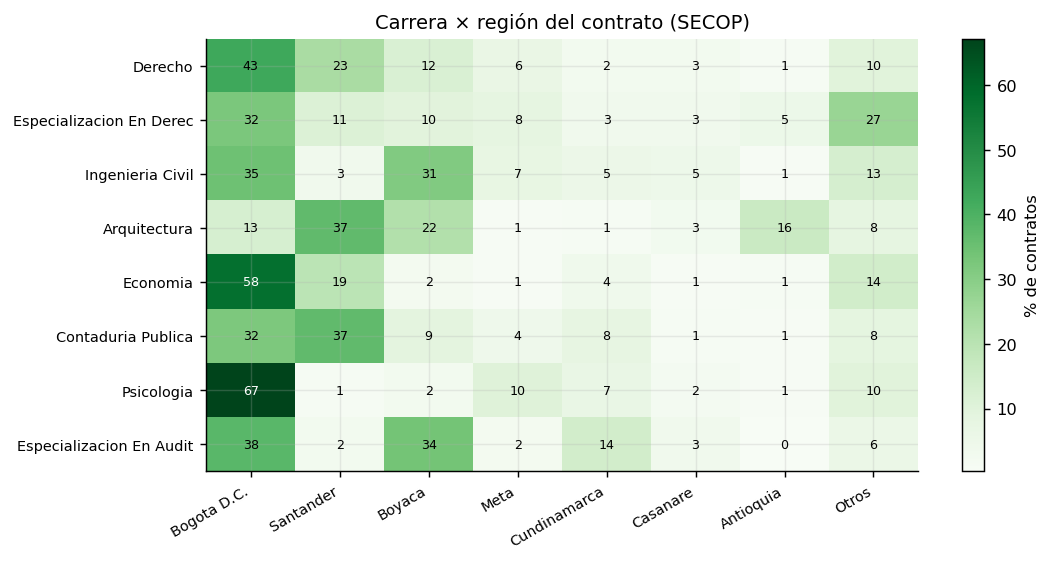
\includegraphics[width=0.92\linewidth]{figs_cruce/S5_secop_carrera_region.png}
\caption{Distribución regional de los contratos por carrera (\% de contratos por fila). El Derecho es la profesión de mayor alcance nacional.}\label{fig:secopcarrerareg}\end{figure}

\subsection{Síntesis del capítulo}
\begin{cajahallazgo}
El graduado tomasino se vincula con el Estado, ante todo, como prestador individual de servicios ---el 92,7\,\% de los contratos---, contratado de forma directa o por régimen especial y mayoritariamente por entidades territoriales, aunque el gran valor resida en unos pocos vínculos nacionales y en un puñado de megacontratos atípicos. La contratación nace en el Derecho y se extiende a las ingenierías, la arquitectura y la salud, con el posgrado como llave hacia contratos de mayor cuantía. El objeto contratado, una vez apartado el genérico administrativo, devuelve la firma disciplinar de cada profesión, y toda la huella aparece territorialmente arraigada: cada carrera contrata sobre todo en la región de su sede, siendo el Derecho la de mayor proyección nacional.
\end{cajahallazgo}

\noindent Queda, no obstante, una frontera por ampliar. El cruce con el SECOP~II que permitió recuperar el UNSPSC cubre solo los contratos electrónicos ---cerca del 39\,\% del total---, de modo que la lectura por objeto, aunque reveladora, descansa sobre una fracción de la contratación. Extender esa recuperación a la totalidad de los contratos, depurando además los megacontratos atípicos por documento, es la continuación natural de este capítulo.
